\documentclass{article}
\usepackage{graphicx}
\usepackage{geometry}
\geometry{margin=1in}

\title{Report on Faast-A-Faas-Framework}
\author{Arijit Saha (210050017) and Aryan Mathe (210050021)}
\date{}

\begin{document}
\maketitle

\section{Introduction}
Faast-A-Faas-Framework is a project designed to evaluate and compare different
cluster configurations for Function as a Service (FaaS) platforms. The goal is
to analyze performance metrics such as response time and resource
utilization across various setups. This report provides an overview of the
project's approach, including the types of clusters tested, the workloads used
for evaluation, and instructions for setting up and running experiments. By
offering insights into the impact of different configurations, this project
aims to guide best practices for optimizing serverless infrastructure

\section{Cluster Configurations}
The project considers the following cluster configurations:

\subsection{Single Pod Cluster}
\nobreak
\vspace{-30px}
\begin{figure}[h]
    \begin{minipage}[t]{0.6\textwidth}
        \vspace{-120px}
        This configuration consists of a single pod with a single container deployed on
        a single-node cluster. The pod hosts the FaaS service, and all incoming
        requests are directed to the single container within the pod. This simple setup
        serves as a baseline for comparison with other configurations.
    \end{minipage}
    \hfill
    \begin{minipage}[b]{0.4\textwidth}
        %\vspace{-20px}
        \centering
        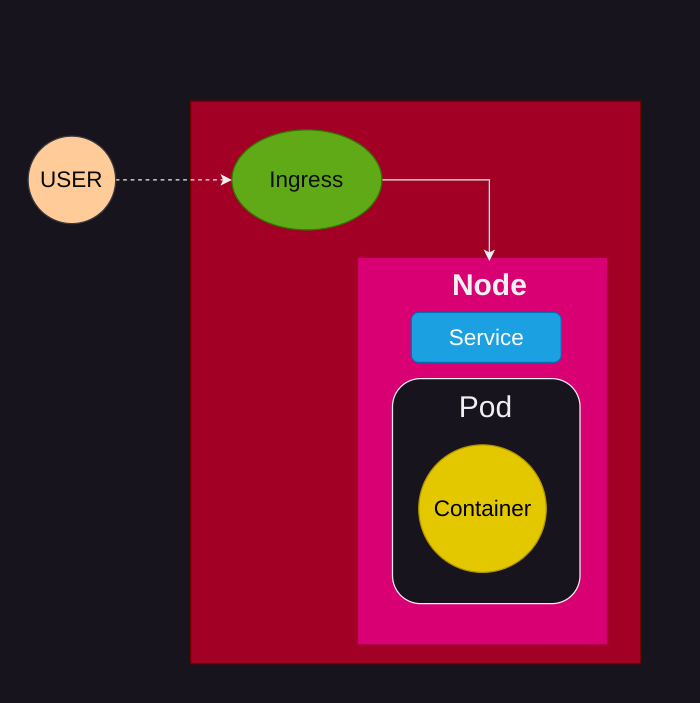
\includegraphics[width=0.7\textwidth]{../images/single_pod.png}
        \caption{Single Pod Cluster}
        \label{fig:single_pod_cluster}
    \end{minipage}
\end{figure}

\vspace{-10px}
\subsection{Single Pod with Multi-Container}
\nobreak
\vspace{-30px}
\begin{figure}[h]
    \begin{minipage}[t]{0.6\textwidth}
        \vspace{-120px}
        In this configuration, a single pod contains multiple containers that
        run the FaaS service on a single-node cluster. An Nginx load balancer
        pod is also deployed to route incoming requests to the containers
        within the pod. This setup allows testing the efficiency of using
        multiple containers within a single pod.
    \end{minipage}%
    \hfill
    \begin{minipage}[b]{0.4\textwidth}
        %\vspace{-20px}
        \centering
        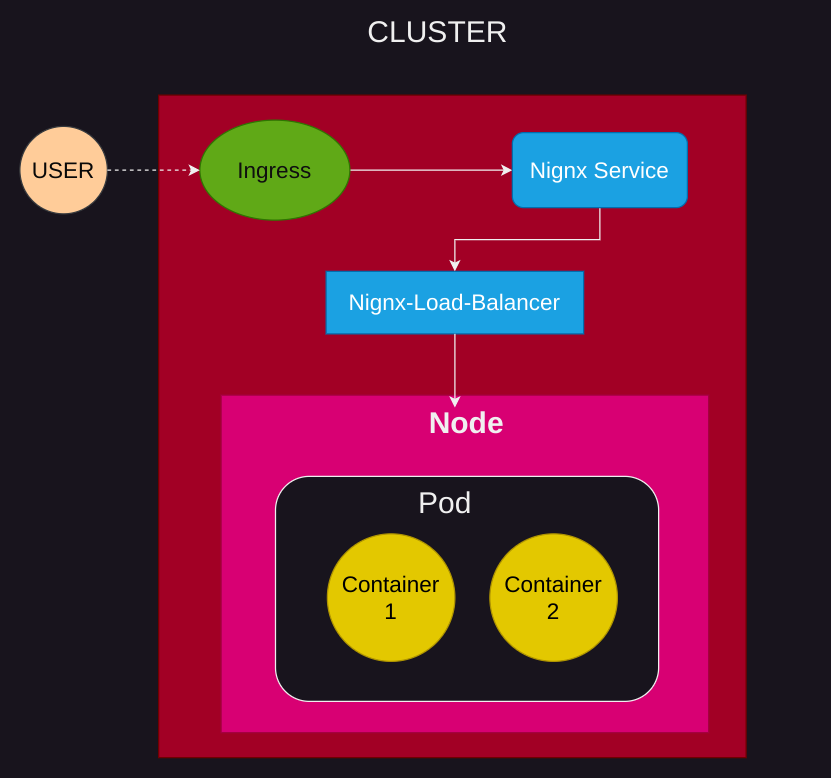
\includegraphics[width=0.7\textwidth]{../images/one_pod_two_container.png}
        \caption{Single Pod with Multi-Container}
        \label{fig:single_pod_multi_container}
    \end{minipage}
\end{figure}
\newpage

\vspace{-10px}
\subsection{Multi-Pod with Single Node}
\nobreak
\vspace{-30px}
\begin{figure}[h]
    \begin{minipage}[t]{0.6\textwidth}
        \vspace{-120px}
        This configuration includes multiple pods, each with one container running the
        FaaS service, deployed on a single node. An Nginx load balancer pod manages
        incoming requests, routing them to the appropriate FaaS service pods. This
        setup tests how multiple pods interact within a single node and the impact of
        load balancing.
    \end{minipage}%
    \hfill
    \begin{minipage}[b]{0.4\textwidth}
        \centering
        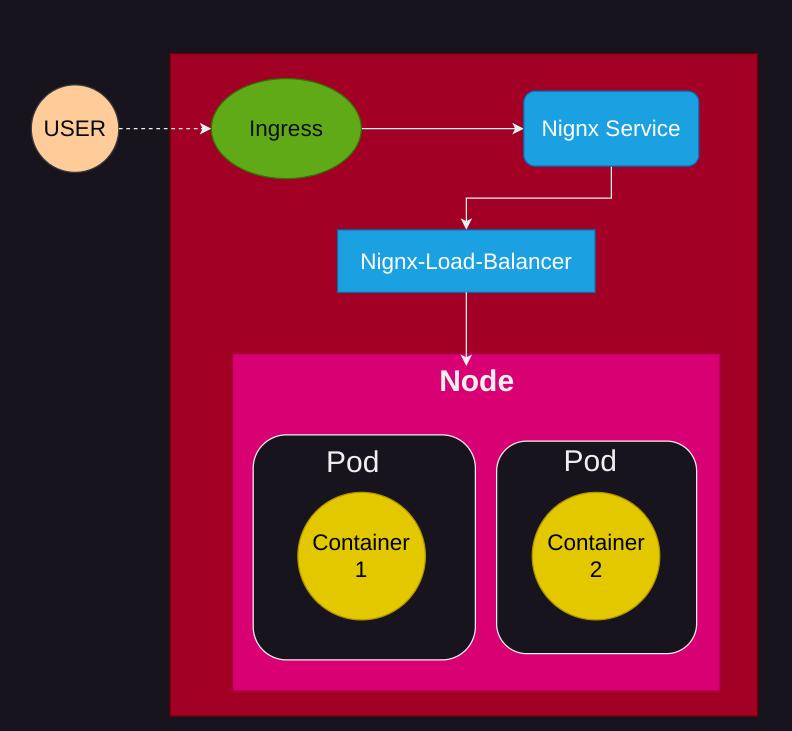
\includegraphics[width=0.7\textwidth]{../images/one_node_two_pod.png}
        \caption{Multi-Pod with Single Node}
        \label{fig:multi_pod_single_node}
    \end{minipage}
\end{figure}

\vspace{-10px}
\subsection{Multi-Pod with Multi-Node}
\nobreak
\vspace{-30px}
\begin{figure}[h]
    \begin{minipage}[t]{0.6\textwidth}
        \vspace{-100px}
        In this configuration, multiple pods are distributed across two different
        nodes, with each pod containing one container running the FaaS service. An
        Nginx load balancer pod manages incoming requests, distributing them evenly
        across the different nodes and their pods. This setup tests how the system
        performs when multiple pods are deployed across multiple nodes.
    \end{minipage}%
    \hfill
    \begin{minipage}[b]{0.4\textwidth}
        \centering
        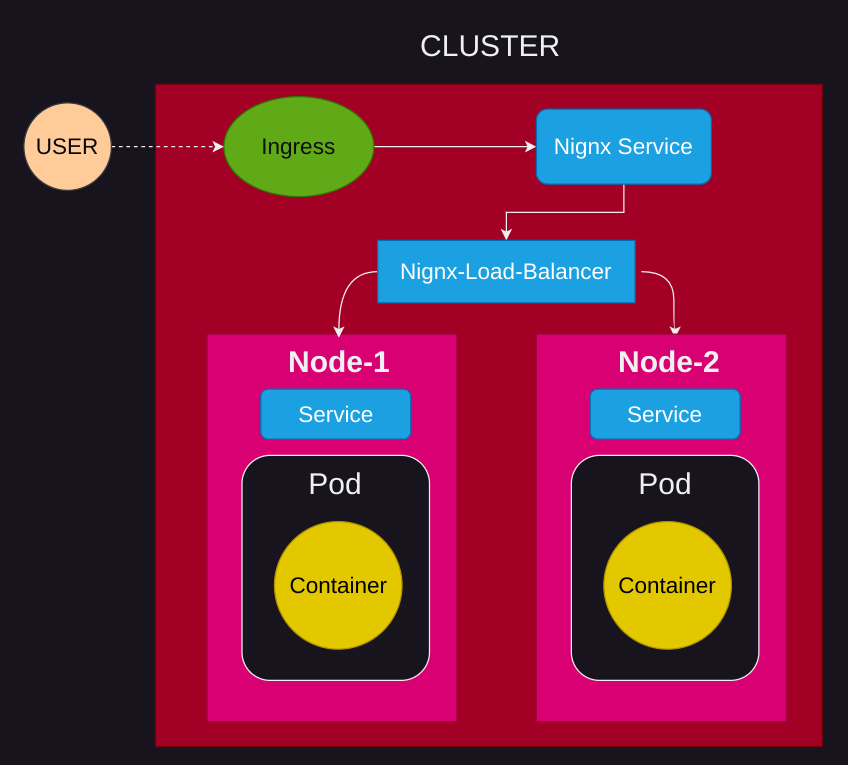
\includegraphics[width=0.7\textwidth]{../images/two_node.png}
        \caption{Multi-Pod with Multi-Node}
        \label{fig:multi_pod_multi_node}
    \end{minipage}
\end{figure}


\vspace{-10px}
\subsection{Horizontal Pod Autoscaler (HPA)}
\nobreak
\vspace{-30px}
\begin{figure}[h]
    \begin{minipage}[t]{0.6\textwidth}
        \vspace{-120px}
        The Horizontal Pod Autoscaler (HPA) is a Kubernetes feature that automatically
        scales the number of pods in response to changes in resource utilization or
        other metrics. In this configuration, multiple pods (initially one) are
        deployed on a single node. The HPA monitors resource usage (such as CPU or
        memory) and dynamically adjusts the number of pods based on predefined
        thresholds, ensuring efficient resource usage and consistent performance.
    \end{minipage}%
    \hfill
    \begin{minipage}[b]{0.4\textwidth}
        \centering
        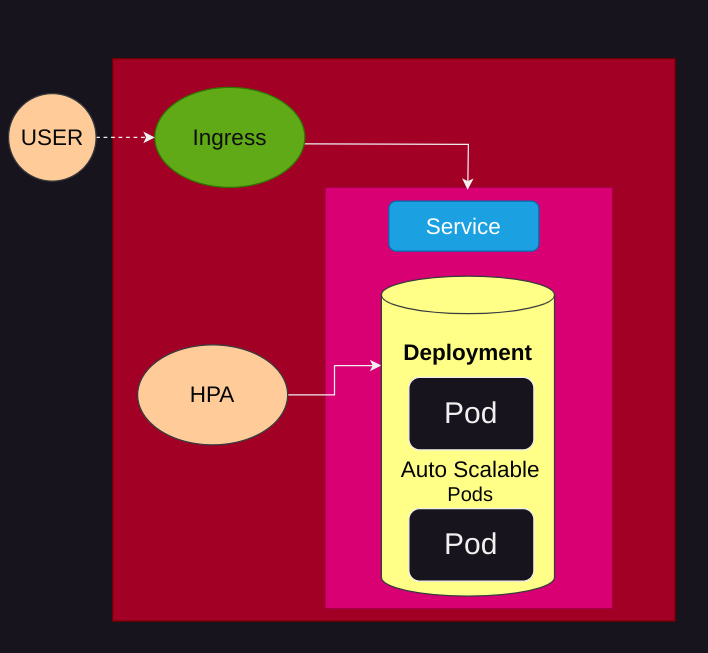
\includegraphics[width=0.7\textwidth]{../images/hpa.png}
        \caption{Horizontal Pod Autoscaler}
        \label{fig:hpa}
    \end{minipage}
\end{figure}

\newpage
\vspace{-10px}
\subsection{Vertical Pod Autoscaler (VPA)}
\nobreak
\vspace{-30px}
\begin{figure}[h]
    \begin{minipage}[t]{0.6\textwidth}
        \vspace{-120px}
        The Vertical Pod Autoscaler (VPA) is a Kubernetes feature that adjusts the
        resource limits and requests of a pod based on its actual usage. In this
        configuration, a single pod is deployed with VPA enabled in a single-node
        cluster. The VPA monitors the pod's resource usage and dynamically adjusts its
        resource requests and limits to ensure optimal performance and resource
        efficiency.
    \end{minipage}%
    \hfill
    \begin{minipage}[b]{0.4\textwidth}
        \centering
        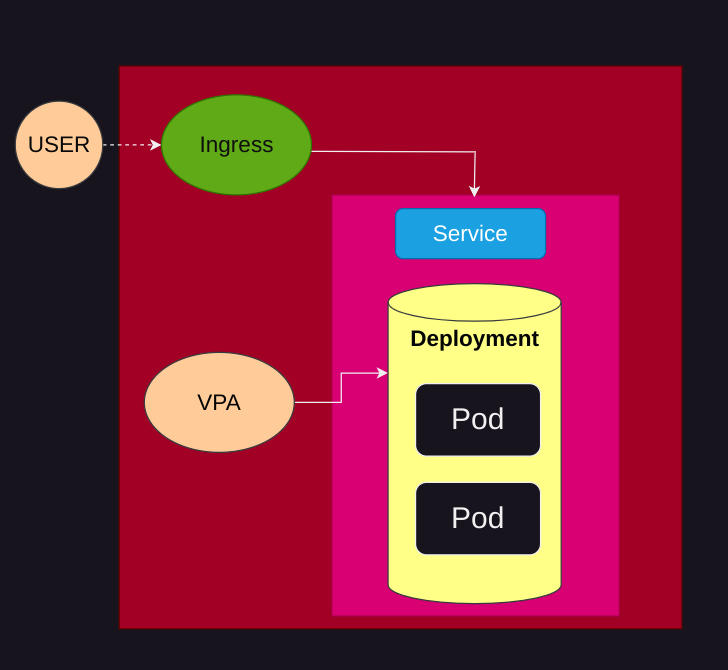
\includegraphics[width=0.7\textwidth]{../images/vpa.png}
        \caption{Vertical Pod Autoscaler}
        \label{fig:vpa}
    \end{minipage}
\end{figure}


\section{Metrics}
This section discusses the metrics used to evaluate the performance and resource utilization of the Function as a Service (FaaS) platform across different cluster configurations. The two main types of workloads tested were a simple loop and a large Lorem Ipsum generator.

\begin{itemize}
    \item \textbf{Responce Time:} A Python script was used to measure response time in three phases:
        Sends 500 individual requests one at a time and records the average response time.
        Sends 500 groups of 10 simultaneous requests and records the average response time for each group.
        Sends 500 groups of 50 simultaneous requests and records the average response time for each group.
This approach allows us to evaluate how each configuration performs under different levels of request concurrency, providing insights into the scalability and efficiency of the system.
 
\end{itemize}


\subsection{Resource Utilization (CPU and Memory)}
Resource utilization is another important aspect of evaluating FaaS services:

\begin{itemize}
    \item \textbf{CPU Usage:} The amount of CPU resources consumed by the FaaS service. Lower CPU usage is preferred as it indicates efficient use of processing power.
    \item \textbf{Memory Usage:} The amount of memory consumed by the FaaS service. Lower memory usage is desirable as it implies efficient use of available memory resources.
\end{itemize}

Resource usage was measured using the Kubernetes `metrics-server` API, which provides real-time data on the CPU and memory usage of pods and containers within the cluster. This data was collected and analyzed for each cluster configuration.
\newpage


\section{Requirements}
To run the experiments, the following tools need to be installed:

\begin{itemize}
   \item docker
   \item kubectl
   \item minikube
   \item helm
\end{itemize}

\section{Running Instructions for Setting up a Cluster Environment}
To set up the environment for running cluster configurations, run the following command:

\begin{verbatim}
bash setup.sh
\end{verbatim}

The supported app-types based on the cluster configurations defined above are:

\begin{verbatim}
single-pod  two-pod-same-node  two-pod-diff-node  hpa  vpa  two-container
\end{verbatim}

%To set up the requirements for running clusters, run the following command with the appropriate `<app_type>`:

\begin{verbatim}
bash deploy_app.sh <app_name> <app_type> <docker_image_name> <python-app-file> <requirements-file> <port> <map_url>
\end{verbatim}

\section{Generating Analysis Results}
To generate analysis results, follow these steps:

\begin{enumerate}
   \item Set up the `metrics-server` REST-API by running the following command in two different terminal windows:
   
   \begin{verbatim}
   minikube dashboard --port=20000
   \end{verbatim}
   
   \item Run the following command to perform the analysis for different cluster configurations and generate logs for response-time and resource utilization:
   
   \begin{verbatim}
   bash src/analysis/perform_analysis.sh <host> <url> <app-type> <app-name>
   \end{verbatim}
   
   This will generate logs for response-time and resource utilization based on the defined workload. The file names will be in the following format:
   
   \begin{verbatim}
   <logs-dir>/<app-name>-<app-type>-response_time.csv
   <logs-dir>/<app-name>-<app-type>-resource_usage.csv
   \end{verbatim}
   
   \item Execute the following Python file to generate plots for the analysis:
   
   \begin{verbatim}
   python3 analysis/get_plot_from_log.py
   usage: script to generate plot from log files [-h] --app-type APP_TYPE
                                                 [--response-log RESPONSE_LOG]
                                                 [--resources-log RESOURCES_LOG] --output-folder
                                                 OUTPUT_FOLDER --app-name APP_NAME

   options:
     -h, --help            show this help message and exit
     --app-type APP_TYPE   single-pod/two-pod-same-node/two-pod-diff-node/hpa/vpa/two-container
     --response-log RESPONSE_LOG
     --resources-log RESOURCES_LOG
     --output-folder OUTPUT_FOLDER
     --app-name APP_NAME
   \end{verbatim}
\end{enumerate}

\section{Analysis}
\subsection{HPA}
\subsubsection{HPA cpu-utilization}
\begin{figure}[h]
    \begin{minipage}[t]{0.5\textwidth}
        \centering
        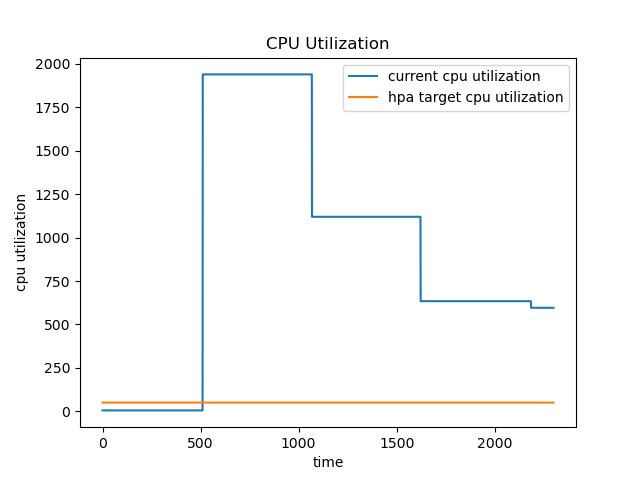
\includegraphics[width=0.9\textwidth]{../sample_results/loop/hpa/cpu-utilization-hpa.png}
        \caption{Loop}
    \end{minipage}
    \hfill
    \begin{minipage}[t]{0.5\textwidth}
        \centering
        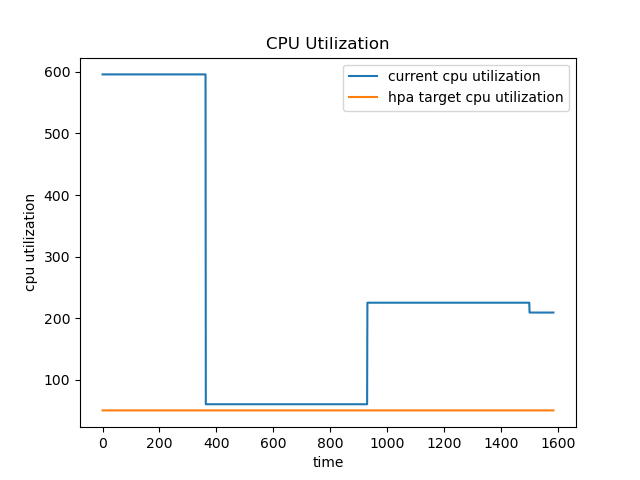
\includegraphics[width=0.9\textwidth]{../sample_results/lorem/hpa/cpu-utilization-hpa.png}
        \caption{Lorem}
    \end{minipage}
\end{figure}
\begin{itemize}
    \item Initial CPU utilization for the HPA configuration is very high due to the limited number of pods available at the start.
    \item As the HPA scales out and increases the number of pods, the workload is distributed across more pods.
    \item Consequently, the CPU utilization per pod decreases over time as more pods are added to handle incoming requests.
    \item This adaptive scaling helps maintain performance while balancing resource usage efficiently.
\end{itemize}

\noindent Below is the replica count graph that illustrates the increase in the number of pods over time, supporting the trend of decreasing CPU utilization per pod:

\begin{figure}[h]
    \begin{minipage}[t]{0.5\textwidth}
        \centering
        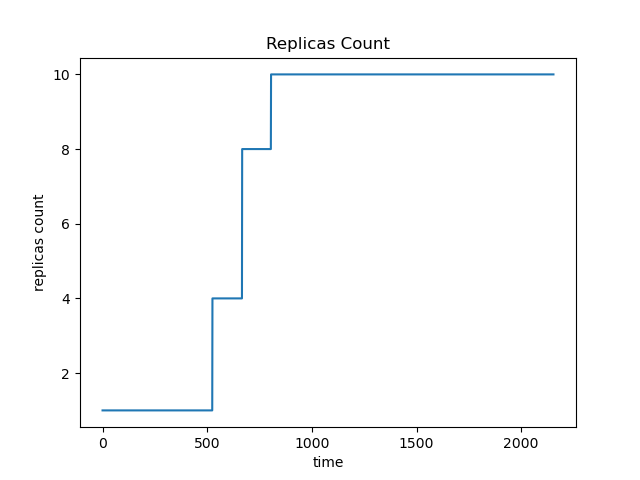
\includegraphics[width=0.9\textwidth]{../sample_results/loop/hpa/replicas-count-hpa.png}
        \caption{Loop}
    \end{minipage}
    \hfill
    \begin{minipage}[t]{0.5\textwidth}
        \centering
        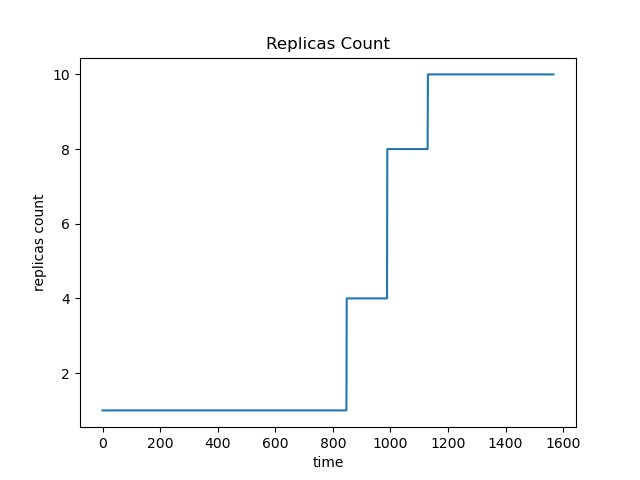
\includegraphics[width=0.9\textwidth]{../sample_results/lorem/hpa/replicas-count-hpa.png}
        \caption{Lorem}
    \end{minipage}
\end{figure}

\subsubsection{HPA Response Time Observations}
\begin{itemize}
    \item Initial response times in the HPA configuration may be higher due to limited pod availability at the start.
    \item As HPA scales out the number of pods in response to increased load, response times start to decrease.
    \item The additional pods allow the service to handle more requests concurrently, resulting in improved response times.
    \item HPA helps maintain consistent response times even as demand fluctuates, by adjusting the number of pods to match the workload.
\end{itemize}

\noindent Below is the response time for HPA.

\begin{figure}[h]
    \begin{minipage}[t]{0.5\textwidth}
        \centering
        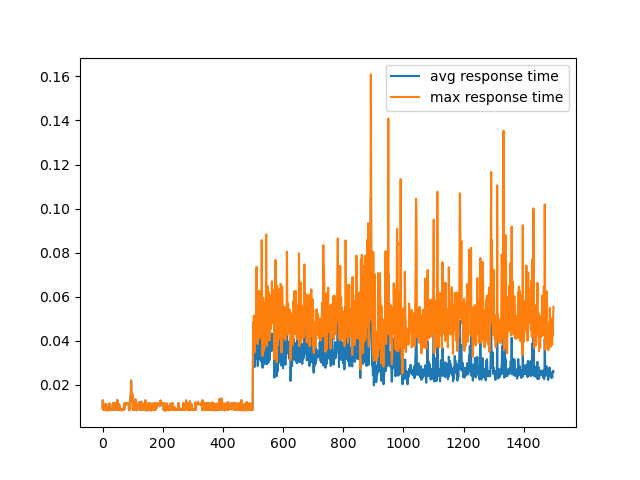
\includegraphics[width=0.9\textwidth]{../sample_results/loop/hpa/response-time-hpa-hpa.png}
        \caption{Loop}
    \end{minipage}
    \hfill
    \begin{minipage}[t]{0.5\textwidth}
        \centering
        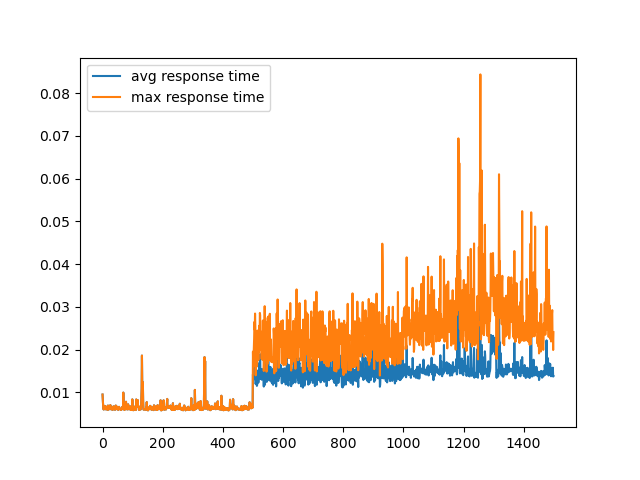
\includegraphics[width=0.9\textwidth]{../sample_results/lorem/hpa/response-time-hpa-hpa.png}
        \caption{Lorem}
    \end{minipage}
\end{figure}


\subsection{VPA}
\subsubsection{VPA CPU Utilization}
\begin{itemize}
    \item VPA initially allocates CPU resources based on current requirements but can increase or decrease them dynamically.
    \item As demand changes, VPA adjusts CPU allocations, potentially causing spikes or dips in utilization as resources are adapted.
    \item These adjustments aim to maintain efficient resource usage and consistent application performance.
\end{itemize}

\noindent Below is the graph that illustrates the adjustments in resource allocation for VPA:

\begin{figure}[h]
    \begin{minipage}[t]{0.5\textwidth}
        \centering
        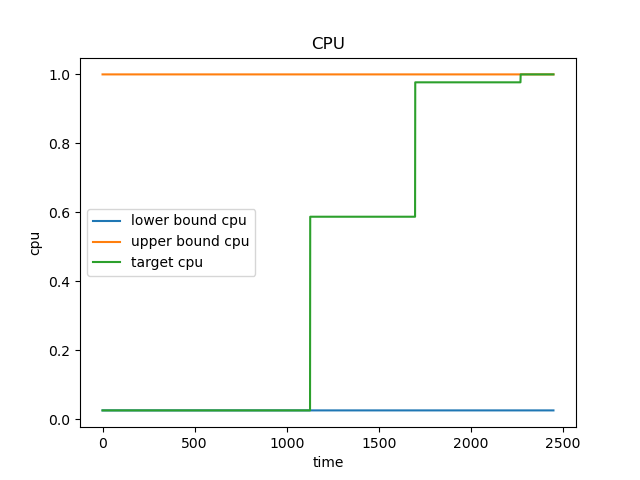
\includegraphics[width=0.9\textwidth]{../sample_results/loop/vpa/cpu-utilization-vpa.png}
        \caption{Loop}
    \end{minipage}
    \hfill
    \begin{minipage}[t]{0.5\textwidth}
        \centering
        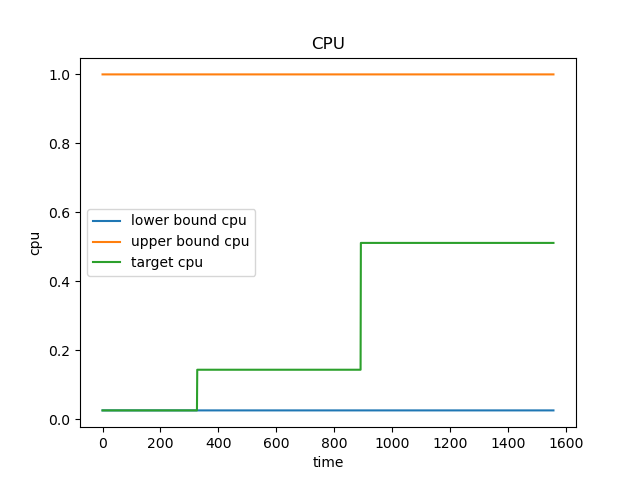
\includegraphics[width=0.9\textwidth]{../sample_results/lorem/vpa/cpu-utilization-vpa.png}
        \caption{Lorem}
    \end{minipage}
\end{figure}
\newpage
\subsubsection{VPA Response Time Observations}
\begin{itemize}
    \item Response times in the VPA configuration can vary as resources are adjusted to meet demand.
    \item Dynamic adjustments in pod resources can lead to fluctuations in response times.
    \item As the VPA optimizes CPU allocations, response times may stabilize, especially when demand is consistent.
    \item VPA aims to balance resource utilization with consistent response times, adapting to varying workloads.
\end{itemize}

\noindent Below are the response time graphs for VPA:

\begin{figure}[h]
    \begin{minipage}[t]{0.5\textwidth}
        \centering
        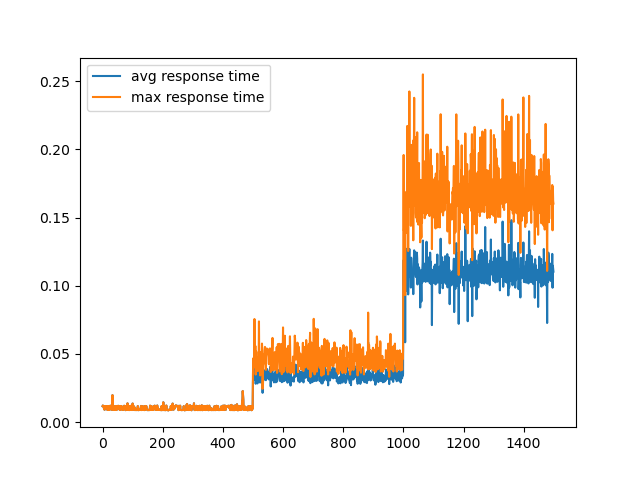
\includegraphics[width=0.9\textwidth]{../sample_results/loop/vpa/response-time-vpa-vpa.png}
        \caption{Loop}
    \end{minipage}
    \hfill
    \begin{minipage}[t]{0.5\textwidth}
        \centering
        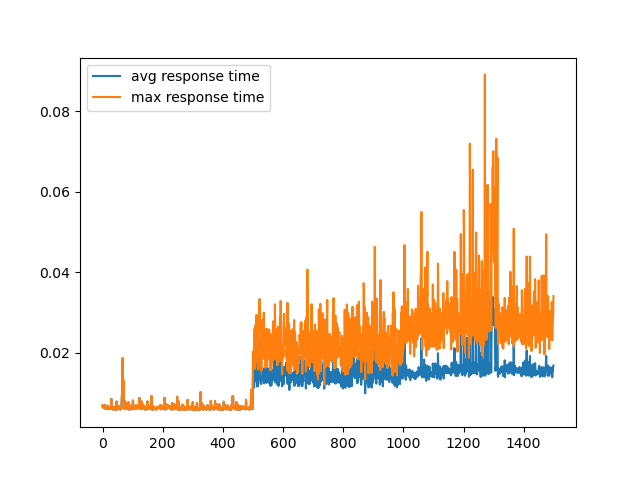
\includegraphics[width=0.9\textwidth]{../sample_results/lorem/vpa/response-time-vpa-vpa.png}
        \caption{Lorem}
    \end{minipage}
\end{figure}

\newpage
\subsubsection{VPA Memory Utilization}
\begin{figure}[h]
    \begin{minipage}[t]{0.5\textwidth}
        \centering
        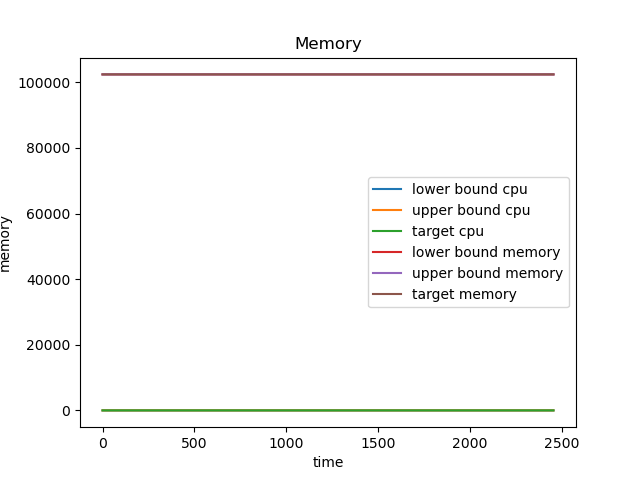
\includegraphics[width=0.9\textwidth]{../sample_results/loop/vpa/mem-utilization-vpa.png}
        \caption{Loop}
    \end{minipage}
    \hfill
    \begin{minipage}[t]{0.5\textwidth}
        \centering
        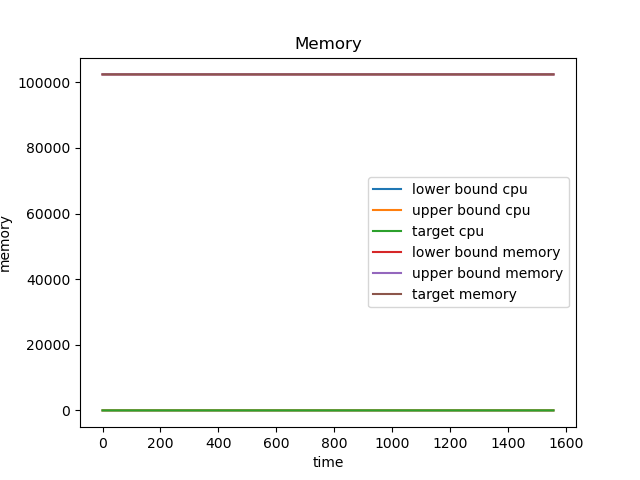
\includegraphics[width=0.9\textwidth]{../sample_results/lorem/vpa/mem-utilization-vpa.png}
        \caption{Lorem}
    \end{minipage}
\end{figure}

\begin{itemize}
    \item VPA manages memory allocations dynamically, adjusting resources according to application needs.
    \item Initial memory usage may vary based on initial resource requests set by VPA.
    \item As the VPA adjusts memory allocations, memory utilization stabilizes according to application requirements.
    \item This adaptive approach optimizes memory usage and aims to maintain consistent application performance.
\end{itemize}


\subsection{Single Pod}
\subsubsection{Single Pod CPU Utilization}
\begin{itemize}
    \item CPU utilization in the Single Pod configuration can be relatively stable, as all workload is handled by a single pod.
    \item The pod may experience higher CPU usage during peak demand since it manages all requests.
    \item Over time, as workloads fluctuate, CPU usage may stabilize as the single pod adjusts to the demand.
\end{itemize}

\noindent Below is the graph that illustrates the CPU utilization for Single Pod:

\begin{figure}[h]
    \begin{minipage}[t]{0.5\textwidth}
        \centering
        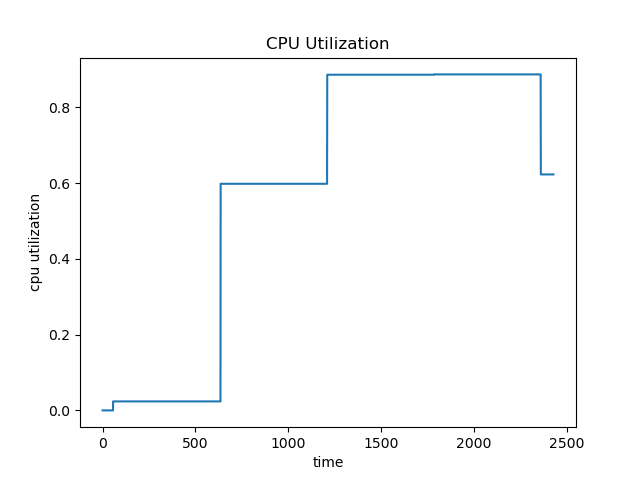
\includegraphics[width=0.9\textwidth]{../sample_results/loop/single-pod/cpu-utilization-single-pod.png}
        \caption{Loop}
    \end{minipage}
    \hfill
    \begin{minipage}[t]{0.5\textwidth}
        \centering
        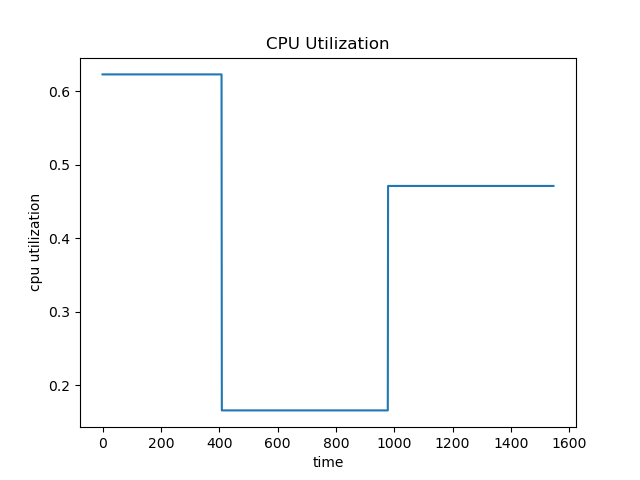
\includegraphics[width=0.9\textwidth]{../sample_results/lorem/single-pod/cpu-utilization-single-pod.png}
        \caption{Lorem}
    \end{minipage}
\end{figure}

\newpage
\subsubsection{Single Pod Response Time Observations}
\begin{itemize}
    \item Response times in the Single Pod configuration can be consistent, as a single pod handles all requests.
    \item Under heavy load, response times may increase due to the single pod being responsible for all tasks.
    \item As workloads stabilize, response times tend to remain steady, provided the pod is not overwhelmed.
\end{itemize}

\noindent Below are the response time graphs for Single Pod:

\begin{figure}[h]
    \begin{minipage}[t]{0.5\textwidth}
        \centering
        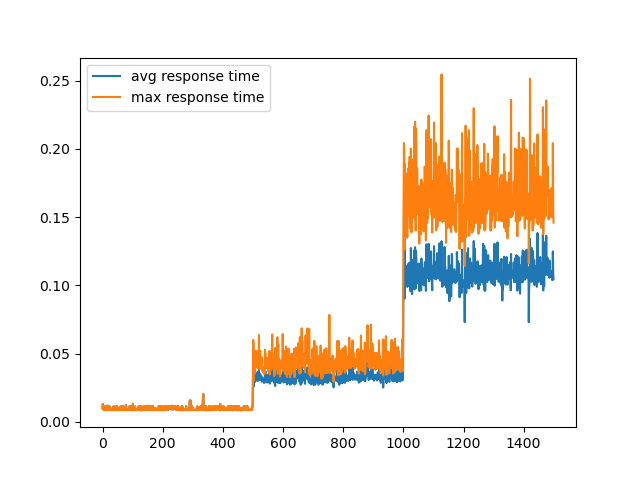
\includegraphics[width=0.9\textwidth]{../sample_results/loop/single-pod/response-time-single-pod-single-pod.png}
        \caption{Loop}
    \end{minipage}
    \hfill
    \begin{minipage}[t]{0.5\textwidth}
        \centering
        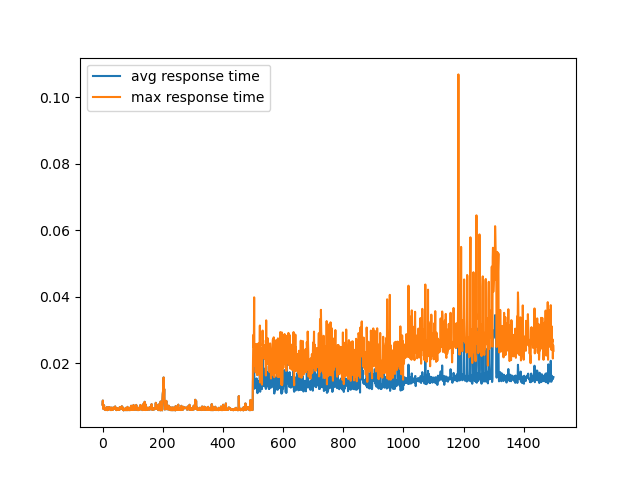
\includegraphics[width=0.9\textwidth]{../sample_results/lorem/single-pod/response-time-single-pod-single-pod.png}
        \caption{Lorem}
    \end{minipage}
\end{figure}

\newpage
\subsubsection{Single Pod Memory Utilization}
\begin{figure}[h]
    \begin{minipage}[t]{0.5\textwidth}
        \centering
        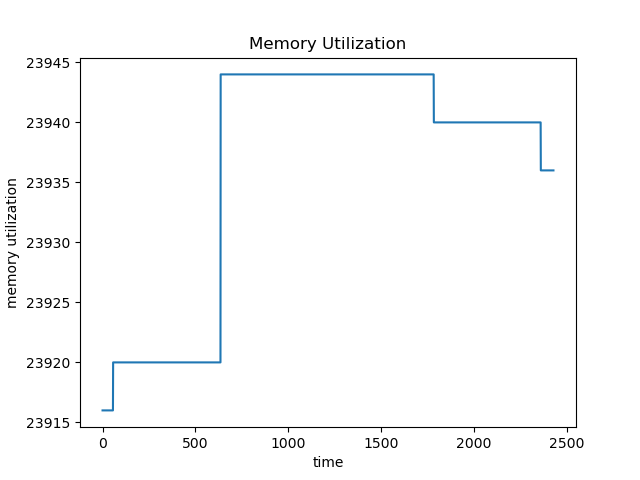
\includegraphics[width=0.9\textwidth]{../sample_results/loop/single-pod/mem-utilization-single-pod.png}
        \caption{Loop}
    \end{minipage}
    \hfill
    \begin{minipage}[t]{0.5\textwidth}
        \centering
        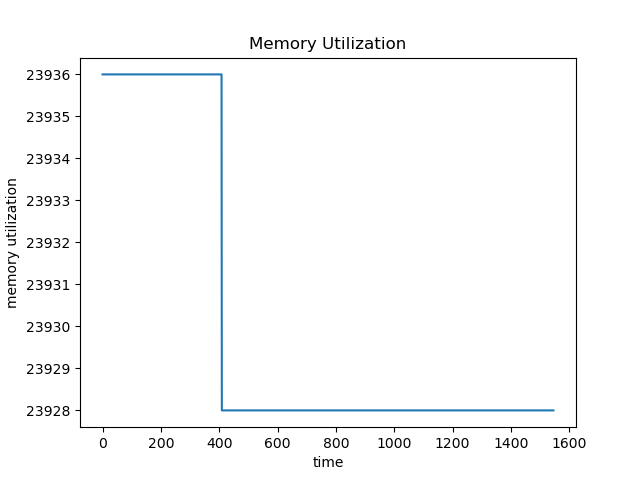
\includegraphics[width=0.9\textwidth]{../sample_results/lorem/single-pod/mem-utilization-single-pod.png}
        \caption{Lorem}
    \end{minipage}
\end{figure}

\begin{itemize}
    \item Memory utilization in the Single Pod configuration can vary based on the complexity of the workloads.
    \item The single pod manages memory allocation for all requests, which can lead to fluctuations in memory usage.
    \item As workloads stabilize, memory utilization tends to even out, provided the single pod is adequately resourced.
\end{itemize}


\subsection{Two-Container}
\subsubsection{Two-Container CPU Utilization}
\begin{itemize}
    \item CPU utilization in the two-container configuration may vary depending on the distribution of workload between the containers.
    \item Both containers can handle requests, potentially balancing the load and leading to lower overall CPU utilization.
    \item Under peak demand, CPU usage may increase as both containers manage incoming requests simultaneously.
\end{itemize}

\noindent Below is the graph that illustrates the CPU utilization for two-container configuration:

\begin{figure}[h]
    \begin{minipage}[t]{0.5\textwidth}
        \centering
        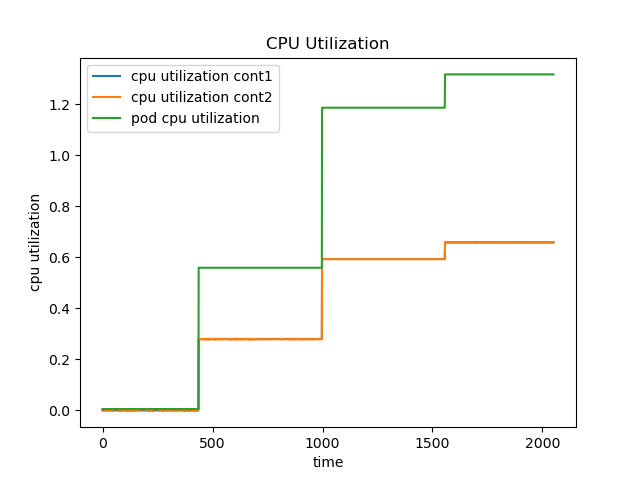
\includegraphics[width=0.9\textwidth]{../sample_results/loop/two-container/cpu-utilization-two-container.png}
        \caption{Loop}
    \end{minipage}
    \hfill
    \begin{minipage}[t]{0.5\textwidth}
        \centering
        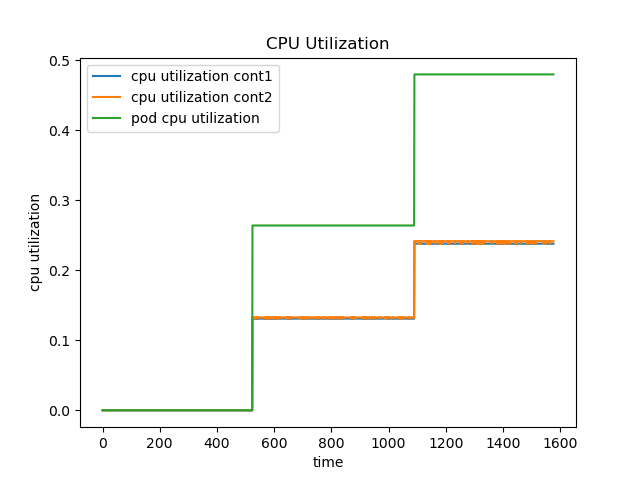
\includegraphics[width=0.9\textwidth]{../sample_results/lorem/two-container/cpu-utilization-two-container.png}
        \caption{Lorem}
    \end{minipage}
\end{figure}

\newpage
\subsubsection{Two-Container Response Time Observations}
\begin{itemize}
    \item Response times in the two-container configuration can be lower, as multiple containers share the workload.
    \item If one container becomes overwhelmed, the other can handle the load, potentially balancing response times.
    \item During peak demand, response times may fluctuate depending on the distribution of requests between the containers.
\end{itemize}

\noindent Below are the response time graphs for two-container configuration:

\begin{figure}[h]
    \begin{minipage}[t]{0.5\textwidth}
        \centering
        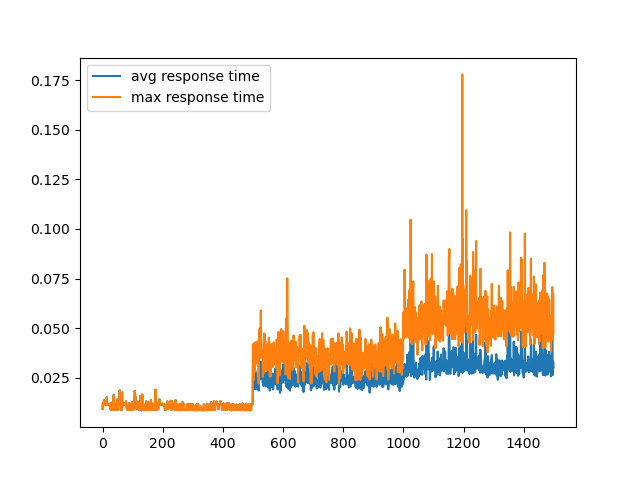
\includegraphics[width=0.9\textwidth]{../sample_results/loop/two-container/response-time-two-container-two-container.png}
        \caption{Loop}
    \end{minipage}
    \hfill
    \begin{minipage}[t]{0.5\textwidth}
        \centering
        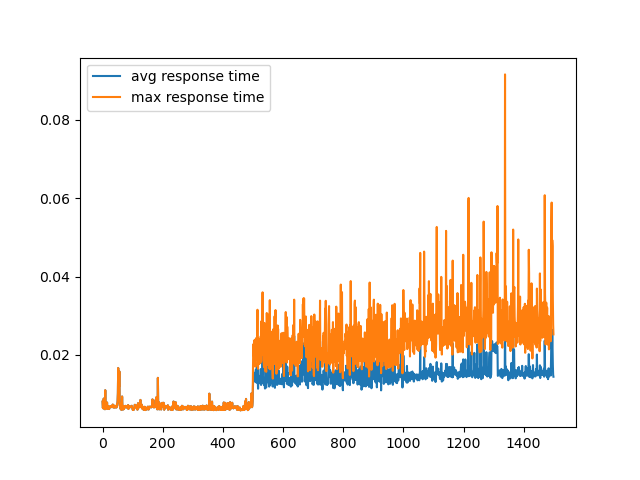
\includegraphics[width=0.9\textwidth]{../sample_results/lorem/two-container/response-time-two-container-two-container.png}
        \caption{Lorem}
    \end{minipage}
\end{figure}

\newpage
\subsubsection{Two-Container Memory Utilization}
\begin{figure}[h]
    \begin{minipage}[t]{0.5\textwidth}
        \centering
        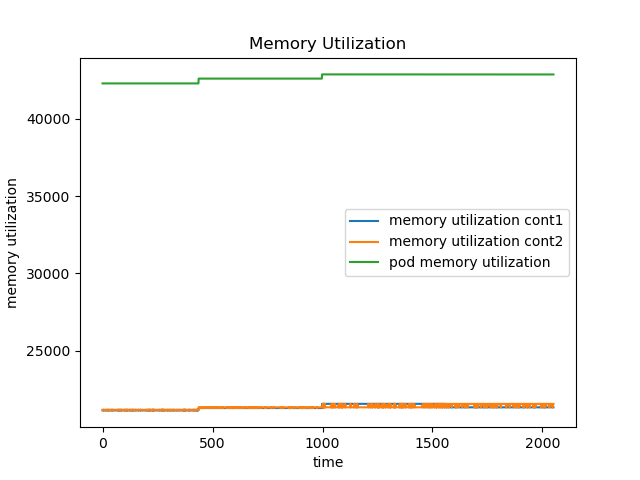
\includegraphics[width=0.9\textwidth]{../sample_results/loop/two-container/mem-utilization-two-container.png}
        \caption{Loop}
    \end{minipage}
    \hfill
    \begin{minipage}[t]{0.5\textwidth}
        \centering
        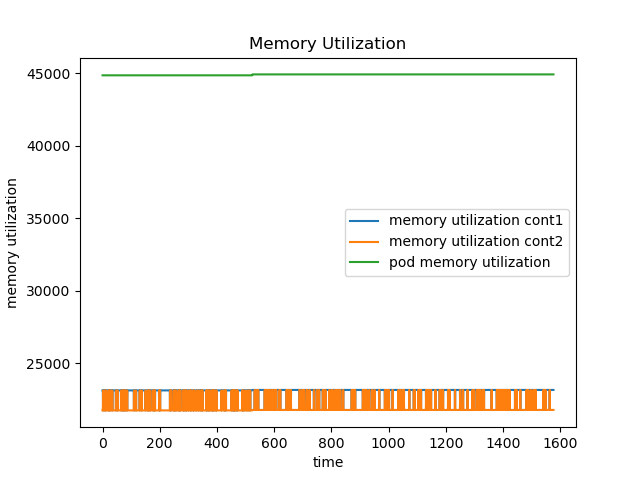
\includegraphics[width=0.9\textwidth]{../sample_results/lorem/two-container/mem-utilization-two-container.png}
        \caption{Lorem}
    \end{minipage}
\end{figure}

\begin{itemize}
    \item Memory utilization in the two-container configuration can vary depending on the memory demands of the workloads.
    \item Each container manages its own memory allocation, which may lead to more efficient usage when workloads are balanced.
    \item As workloads stabilize, memory utilization should even out as both containers manage their respective resources.
\end{itemize}


\subsection{Two Pods Same Node}
\subsubsection{Two Pods Same Node CPU Utilization}
\begin{itemize}
    \item In the two-pods-same-node configuration, CPU utilization may be more stable compared to the single pod setup, as the workload is distributed across two pods.
    \item With two pods handling incoming requests, the load is shared, potentially reducing the CPU usage of each pod.
    \item During peak demand, CPU usage may increase as both pods manage concurrent requests on the same node.
\end{itemize}

\noindent Below is the graph that illustrates the CPU utilization for the two-pods-same-node configuration:

\begin{figure}[h]
    \begin{minipage}[t]{0.5\textwidth}
        \centering
        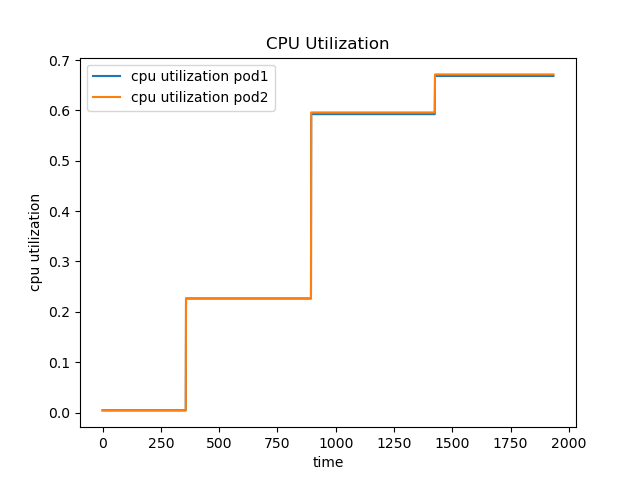
\includegraphics[width=0.9\textwidth]{../sample_results/loop/two-pod-same-node/cpu-utilization-two-pod-same-node.png}
        \caption{Loop}
    \end{minipage}
    \hfill
    \begin{minipage}[t]{0.5\textwidth}
        \centering
        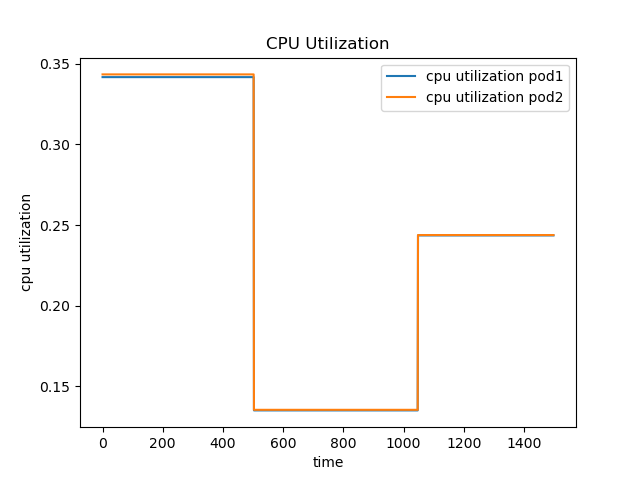
\includegraphics[width=0.9\textwidth]{../sample_results/lorem/two-pod-same-node/cpu-utilization-two-pod-same-node.png}
        \caption{Lorem}
    \end{minipage}
\end{figure}

\newpage
\subsubsection{Two Pods Same Node Response Time Observations}
\begin{itemize}
    \item Response times in the two-pods-same-node configuration can be consistent, as two pods share the workload.
    \item If one pod is under heavy load, the other can manage additional requests, balancing response times.
    \item This setup helps maintain consistent response times as the workload is distributed across both pods.
\end{itemize}

\noindent Below are the response time graphs for the two-pods-same-node configuration:

\begin{figure}[h]
    \begin{minipage}[t]{0.5\textwidth}
        \centering
        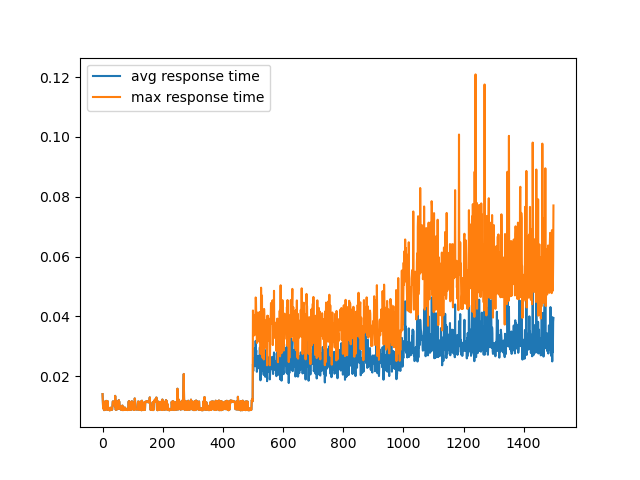
\includegraphics[width=0.9\textwidth]{../sample_results/loop/two-pod-same-node/response-time-two-pod-same-node-two-pod-same-node.png}
        \caption{Loop}
    \end{minipage}
    \hfill
    \begin{minipage}[t]{0.5\textwidth}
        \centering
        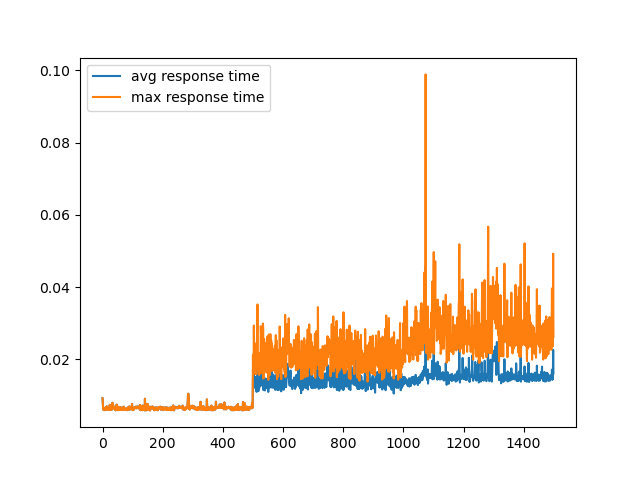
\includegraphics[width=0.9\textwidth]{../sample_results/lorem/two-pod-same-node/response-time-two-pod-same-node-two-pod-same-node.png}
        \caption{Lorem}
    \end{minipage}
\end{figure}

\newpage
\subsubsection{Two Pods Same Node Memory Utilization}
\begin{figure}[h]
    \begin{minipage}[t]{0.5\textwidth}
        \centering
        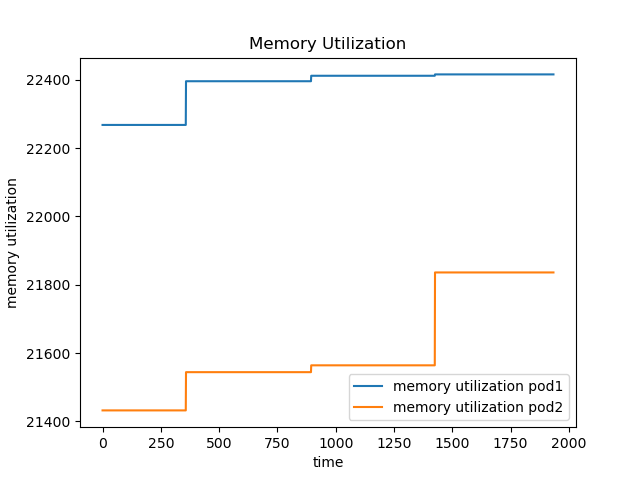
\includegraphics[width=0.9\textwidth]{../sample_results/loop/two-pod-same-node/mem-utilization-two-pod-same-node.png}
        \caption{Loop}
    \end{minipage}
    \hfill
    \begin{minipage}[t]{0.5\textwidth}
        \centering
        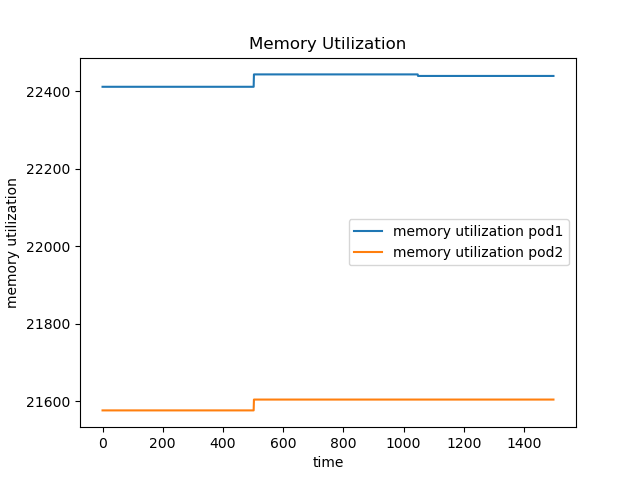
\includegraphics[width=0.9\textwidth]{../sample_results/lorem/two-pod-same-node/mem-utilization-two-pod-same-node.png}
        \caption{Lorem}
    \end{minipage}
\end{figure}

\begin{itemize}
    \item Memory utilization in the two-pods-same-node configuration can vary based on the workloads and the memory requirements of each pod.
    \item Since two pods share the same node, memory usage might be affected by how each pod manages its resources.
    \item As workloads stabilize, memory utilization tends to balance out as both pods handle their own resource management.
\end{itemize}


\subsection{Two Pods Different Node}
\subsubsection{Two Pods Different Node CPU Utilization}
\begin{itemize}
    \item In the two-pod-diff-node configuration, CPU utilization may vary depending on the distribution of workload across the two pods located on different nodes.
    \item Since each pod is on a different node, the workload is distributed evenly, potentially balancing the overall CPU usage across nodes.
    \item CPU utilization may vary as each pod handles its respective requests, but overall utilization may stabilize over time.
\end{itemize}

\noindent Below is the graph that illustrates the CPU utilization for the two-pod-diff-node configuration:

\begin{figure}[h]
    \begin{minipage}[t]{0.5\textwidth}
        \centering
        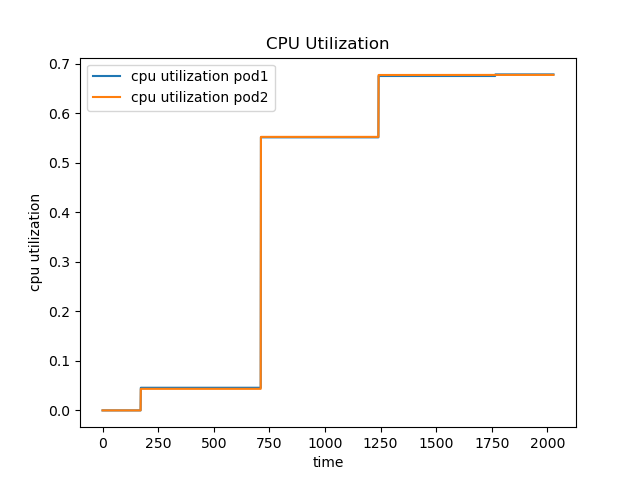
\includegraphics[width=0.9\textwidth]{../sample_results/loop/two-pod-diff-node/cpu-utilization-two-pod-diff-node.png}
        \caption{Loop}
    \end{minipage}
    \hfill
    \begin{minipage}[t]{0.5\textwidth}
        \centering
        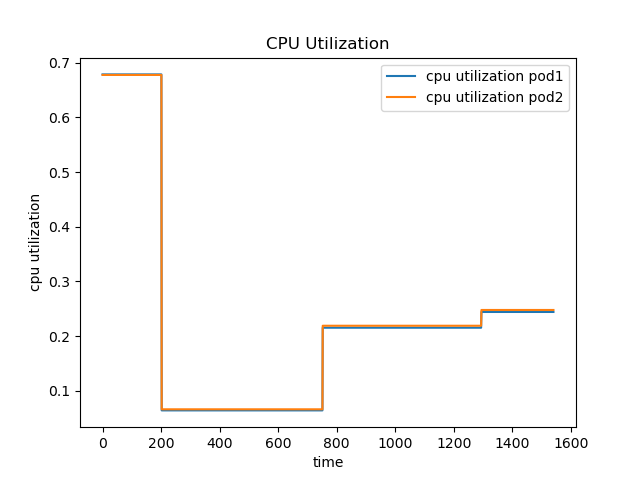
\includegraphics[width=0.9\textwidth]{../sample_results/lorem/two-pod-diff-node/cpu-utilization-two-pod-diff-node.png}
        \caption{Lorem}
    \end{minipage}
\end{figure}

\newpage
\subsubsection{Two Pods Different Node Response Time Observations}
\begin{itemize}
    \item Response times in the two-pod-diff-node configuration may be consistent due to the even distribution of workload across the two pods on different nodes.
    \item The setup allows each pod to handle requests independently, possibly balancing the load and resulting in more consistent response times.
    \item Under peak demand, response times may increase if either pod becomes overwhelmed, but overall, the configuration tends to provide more consistent response times.
\end{itemize}

\noindent Below are the response time graphs for the two-pod-diff-node configuration:

\begin{figure}[h]
    \begin{minipage}[t]{0.5\textwidth}
        \centering
        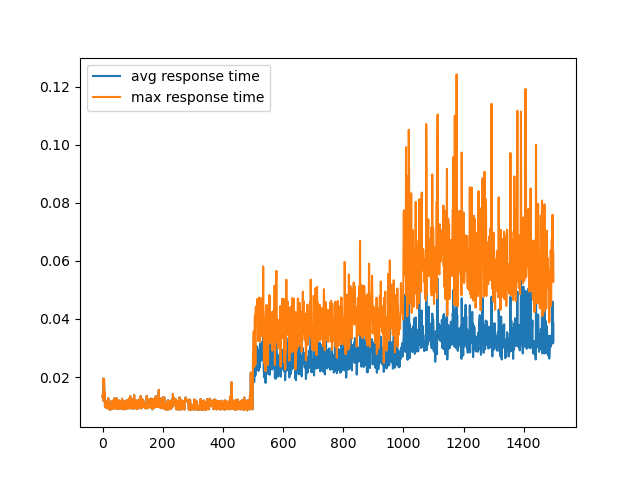
\includegraphics[width=0.9\textwidth]{../sample_results/loop/two-pod-diff-node/response-time-two-pod-diff-node-two-pod-diff-node.png}
        \caption{Loop}
    \end{minipage}
    \hfill
    \begin{minipage}[t]{0.5\textwidth}
        \centering
        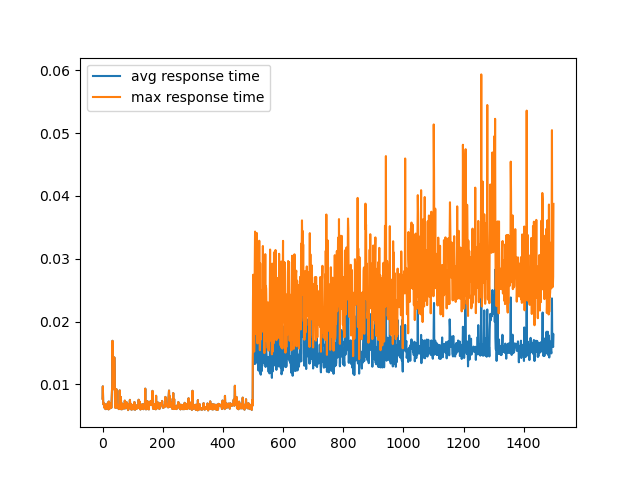
\includegraphics[width=0.9\textwidth]{../sample_results/lorem/two-pod-diff-node/response-time-two-pod-diff-node-two-pod-diff-node.png}
        \caption{Lorem}
    \end{minipage}
\end{figure}

\newpage
\subsubsection{Two Pods Different Node Memory Utilization}
\begin{figure}[h]
    \begin{minipage}[t]{0.5\textwidth}
        \centering
        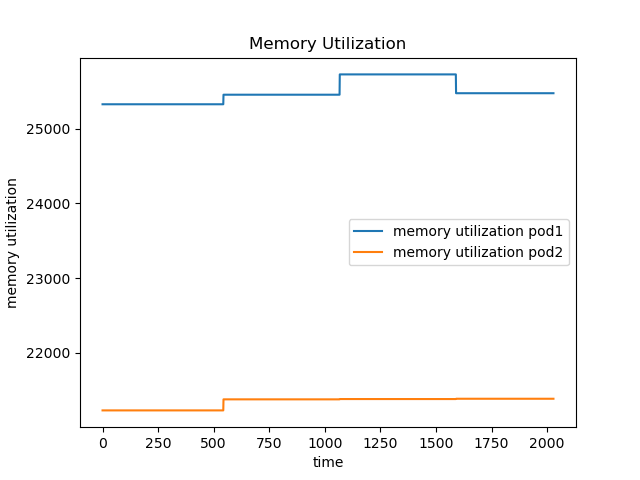
\includegraphics[width=0.9\textwidth]{../sample_results/loop/two-pod-diff-node/mem-utilization-two-pod-diff-node.png}
        \caption{Loop}
    \end{minipage}
    \hfill
    \begin{minipage}[t]{0.5\textwidth}
        \centering
        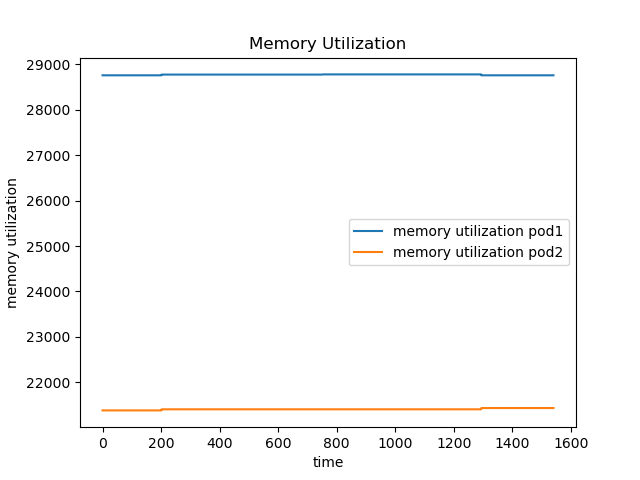
\includegraphics[width=0.9\textwidth]{../sample_results/lorem/two-pod-diff-node/mem-utilization-two-pod-diff-node.png}
        \caption{Lorem}
    \end{minipage}
\end{figure}

\begin{itemize}
    \item Memory utilization in the two-pod-diff-node configuration can vary depending on the memory requirements of each pod on different nodes.
    \item Since the pods are on separate nodes, memory usage is isolated per pod, potentially leading to efficient usage of resources.
    \item As workloads stabilize, memory utilization tends to balance out as each pod manages its own resources independently.
\end{itemize}


\section{Comparison of Average Response Times}

\begin{table}[h]
    \centering
    \caption{Average Response Times across Configurations}
    \begin{tabular}{|l|c|}
        \hline
        \textbf{Configuration} & \textbf{Average Response Time (s)} \\
        \hline
        Horizontal Pod Autoscaler (HPA) & 0.02 - 0.04 \\
        Vertical Pod Autoscaler (VPA) & 0.1 - 0.15 \\
        Single Pod & 0.1 - 0.15 \\
        Two-Container & 0.04 - 0.05 \\
        Two-Pod Same Node & 0.03 - 0.04 \\
        Two-Pod Different Node & 0.04 - 0.045 \\
        \hline
    \end{tabular}
    \label{tab:response_times}
\end{table}

\noindent This table summarizes the average response times across the six configurations:

\begin{itemize}
    \item \textbf{HPA:} Offers the lowest average response time, ranging from 0.02 to 0.04 seconds. This configuration scales out the number of pods effectively to handle incoming requests, resulting in fast response times.
    \item \textbf{VPA:} The average response time for VPA is higher, ranging from 0.1 to 0.15 seconds, possibly due to dynamic adjustments in resource allocation.
    \item \textbf{Single Pod:} Similar to VPA, single pod configurations exhibit an average response time of 0.1 to 0.15 seconds, as a single pod manages all incoming requests.
    \item \textbf{Two-Container:} The two-container configuration offers an average response time between 0.04 and 0.05 seconds. This setup distributes the workload across multiple containers within a single pod, resulting in relatively low response times.
    \item \textbf{Two-Pod Same Node:} This configuration demonstrates average response times between 0.03 and 0.04 seconds, distributing the workload across two pods on a single node for efficient request handling.
    \item \textbf{Two-Pod Different Node:} This setup results in average response times ranging from 0.04 to 0.045 seconds. Distributing the workload across two pods on different nodes may lead to more balanced response times.
\end{itemize}

In summary, HPA demonstrates the lowest average response times, while VPA and single pod setups show higher response times. The other configurations offer varying levels of performance based on how the workload is distributed.


\end{document}
